\documentclass[10pt]{beamer}\usepackage[]{graphicx}\usepackage[]{color}
%% maxwidth is the original width if it is less than linewidth
%% otherwise use linewidth (to make sure the graphics do not exceed the margin)
\makeatletter
\def\maxwidth{ %
  \ifdim\Gin@nat@width>\linewidth
    \linewidth
  \else
    \Gin@nat@width
  \fi
}
\makeatother

\definecolor{fgcolor}{rgb}{0.345, 0.345, 0.345}
\newcommand{\hlnum}[1]{\textcolor[rgb]{0.686,0.059,0.569}{#1}}%
\newcommand{\hlstr}[1]{\textcolor[rgb]{0.192,0.494,0.8}{#1}}%
\newcommand{\hlcom}[1]{\textcolor[rgb]{0.678,0.584,0.686}{\textit{#1}}}%
\newcommand{\hlopt}[1]{\textcolor[rgb]{0,0,0}{#1}}%
\newcommand{\hlstd}[1]{\textcolor[rgb]{0.345,0.345,0.345}{#1}}%
\newcommand{\hlkwa}[1]{\textcolor[rgb]{0.161,0.373,0.58}{\textbf{#1}}}%
\newcommand{\hlkwb}[1]{\textcolor[rgb]{0.69,0.353,0.396}{#1}}%
\newcommand{\hlkwc}[1]{\textcolor[rgb]{0.333,0.667,0.333}{#1}}%
\newcommand{\hlkwd}[1]{\textcolor[rgb]{0.737,0.353,0.396}{\textbf{#1}}}%
\let\hlipl\hlkwb

\usepackage{framed}
\makeatletter
\newenvironment{kframe}{%
 \def\at@end@of@kframe{}%
 \ifinner\ifhmode%
  \def\at@end@of@kframe{\end{minipage}}%
  \begin{minipage}{\columnwidth}%
 \fi\fi%
 \def\FrameCommand##1{\hskip\@totalleftmargin \hskip-\fboxsep
 \colorbox{shadecolor}{##1}\hskip-\fboxsep
     % There is no \\@totalrightmargin, so:
     \hskip-\linewidth \hskip-\@totalleftmargin \hskip\columnwidth}%
 \MakeFramed {\advance\hsize-\width
   \@totalleftmargin\z@ \linewidth\hsize
   \@setminipage}}%
 {\par\unskip\endMakeFramed%
 \at@end@of@kframe}
\makeatother

\definecolor{shadecolor}{rgb}{.97, .97, .97}
\definecolor{messagecolor}{rgb}{0, 0, 0}
\definecolor{warningcolor}{rgb}{1, 0, 1}
\definecolor{errorcolor}{rgb}{1, 0, 0}
\newenvironment{knitrout}{}{} % an empty environment to be redefined in TeX

\usepackage{alltt}
\usepackage{amsmath}
\usepackage{amssymb}
\usepackage{geometry}
\usepackage{graphicx}
\usepackage{url}
\usepackage{bm}

\makeatletter
\let \@sverbatim \@verbatim
\def \@verbatim {\@sverbatim \verbatimplus}
{\catcode`'=13 \gdef \verbatimplus{\catcode`'=13 \chardef '=13 }} 
\makeatother

\newcommand{\AIC}{\text{AIC}}
\newcommand{\BIC}{\text{BIC}}
\newcommand{\RSS}{\text{RSS}}
\newcommand{\hbeta}{\hat{\beta}}
\newcommand{\hsigma}{\hat{\sigma}}
\IfFileExists{upquote.sty}{\usepackage{upquote}}{}
\begin{document}

% --------------------------------------------
\begin{frame}
\large
Lecture 16:\\ 
Variable Selection\\
STAT 632, Spring 2020\\
\end{frame}

% --------------------------------------------
\begin{frame}{Variable Selection}
The process of selecting which predictors to include in a model is referred to as \textbf{variable selection}.\\
\vspace{10pt}

Why should we perform variable selection?
\begin{enumerate}[(1)]
\item \emph{Interpretation}:  A model with fewer variables is easier to interpret and explain.
\vspace{5pt}
\item \emph{Prediction}:  A model with too many predictors can ``over-fit" the data, and perform poorly when making future predictions.
\vspace{5pt}
\item \emph{Cost}: It is cheaper to collect data on fewer variables.
\end{enumerate}
\end{frame}


% --------------------------------------------
\begin{frame}{Backwards Elimination}
One of the simplest methods for variable selection:
\vspace{5pt}
\begin{enumerate}[(1)]
\item Start with the full model that includes all the predictor variables.
\vspace{5pt}
\item Identify the predictor with the largest $p$-value (this is the predictor that is the least statistically significant in the model).
\vspace{5pt}
\begin{enumerate}[(a)]
\item If the $p$-value is large (say, greater than 10\%), remove that predictor and refit the model; then return to step 2.
\vspace{5pt}
\item If the $p$-value is small (say, smaller than 10\%), stop since all the remaining predictors are significant.
\end{enumerate}
\end{enumerate}
\vspace{5pt}
Other cut-offs for the $p$-value can be used such as 5\%.  Generally, smaller cut-offs result in more predictors being eliminated.
\end{frame}

% --------------------------------------------
\begin{frame}{Example: Census Data (1970)}
\begin{itemize}
\item We illustrate this method using U.S. Census Bureau data on 50 states from the 1970s.  This is a base R data set (no package necessary).\footnote{Example from Julian Faraway, \emph{Linear Models with R}, 1st edition, pp. 122--125}
\vspace{5pt}
\item The response variable is \texttt{Life.Exp}, life expectancy in years.
\vspace{5pt}
\item The predictors are:
\begin{itemize}
\item \texttt{Population}: population estimate
\item \texttt{Income}: per capita income
\item \texttt{Illiteracy}: percent illiterate
\item \texttt{Murder}: murder rate per 100,000 population
\item \texttt{HS.Grad}: percent high-school graduates
\item \texttt{Frost}: mean number of days with minimum temperature below freezing in capital city
\item \texttt{Area}: land area in square miles
\end{itemize}
\end{itemize}
\end{frame}

% --------------------------------------------
\begin{frame}[fragile]
\small
\scriptsize
\begin{verbatim}
> statedata <- data.frame(state.x77, row.names=state.abb)

> head(statedata)
   Population Income Illiteracy Life.Exp Murder HS.Grad Frost   Area
AL       3615   3624        2.1    69.05   15.1    41.3    20  50708
AK        365   6315        1.5    69.31   11.3    66.7   152 566432
AZ       2212   4530        1.8    70.55    7.8    58.1    15 113417
AR       2110   3378        1.9    70.66   10.1    39.9    65  51945
CA      21198   5114        1.1    71.71   10.3    62.6    20 156361
CO       2541   4884        0.7    72.06    6.8    63.9   166 103766

> dim(statedata)
[1] 50  8
\end{verbatim}
\end{frame}

% --------------------------------------------
\begin{frame}
\begin{figure}
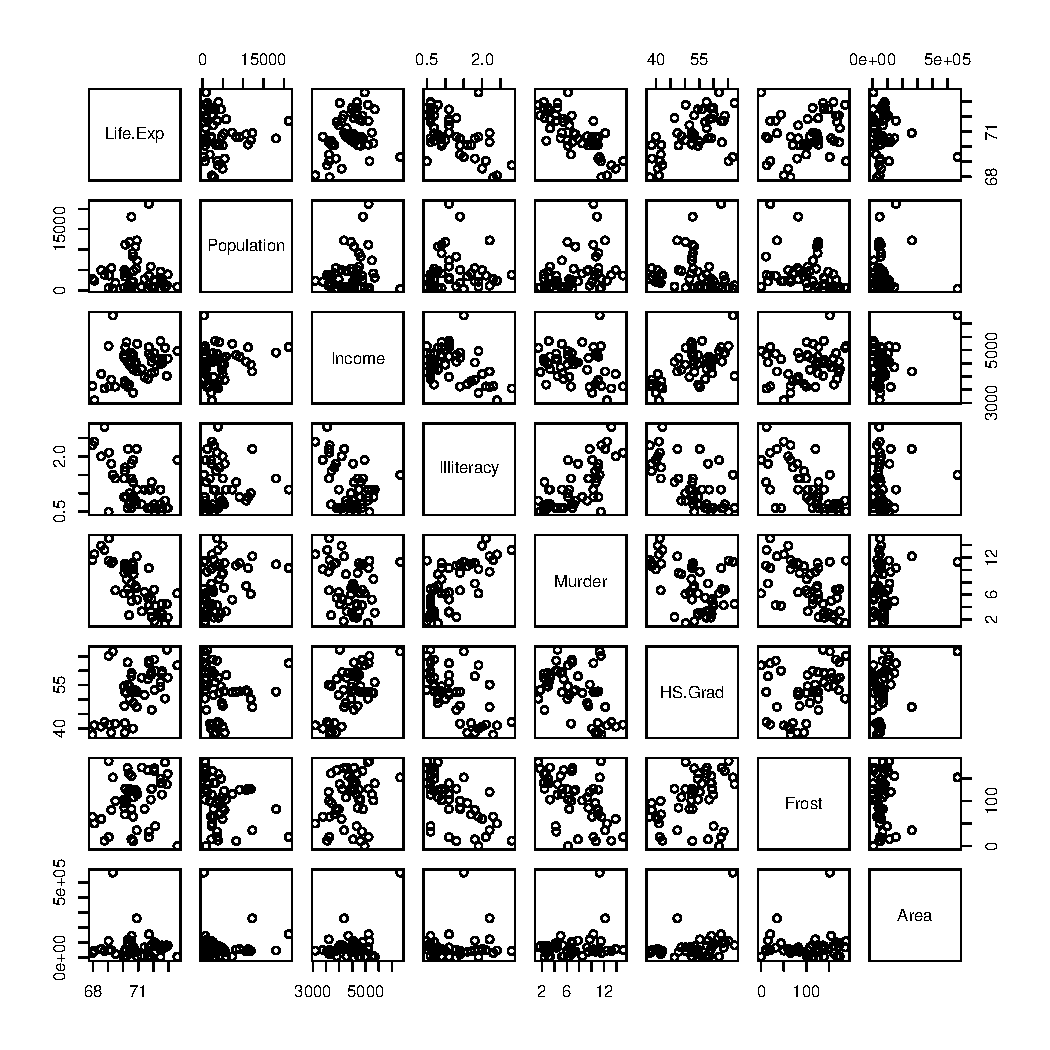
\includegraphics[scale=0.5]{figure/state_pairs.pdf}
\end{figure}
\end{frame}

% --------------------------------------------
\begin{frame}[fragile]
\scriptsize
\begin{verbatim}
> lm1 <- lm(Life.Exp ~ ., data=statedata)
> summary(lm1)

Coefficients:
              Estimate Std. Error t value Pr(>|t|)    
(Intercept)  7.094e+01  1.748e+00  40.586  < 2e-16 ***
Population   5.180e-05  2.919e-05   1.775   0.0832 .  
Income      -2.180e-05  2.444e-04  -0.089   0.9293    
Illiteracy   3.382e-02  3.663e-01   0.092   0.9269    
Murder      -3.011e-01  4.662e-02  -6.459 8.68e-08 ***
HS.Grad      4.893e-02  2.332e-02   2.098   0.0420 *  
Frost       -5.735e-03  3.143e-03  -1.825   0.0752 .  
Area        -7.383e-08  1.668e-06  -0.044   0.9649    
---
Signif. codes:  0 ‘***’ 0.001 ‘**’ 0.01 ‘*’ 0.05 ‘.’ 0.1 ‘ ’ 1

Residual standard error: 0.7448 on 42 degrees of freedom
Multiple R-squared:  0.7362,	Adjusted R-squared:  0.6922 
F-statistic: 16.74 on 7 and 42 DF,  p-value: 2.534e-10
\end{verbatim}
\end{frame}

% --------------------------------------------
\begin{frame}[fragile]
\scriptsize
\begin{verbatim}
> lm2 <- update(lm1, ~ . - Area)
> summary(lm2)

Coefficients:
               Estimate  Std. Error t value Pr(>|t|)    
(Intercept) 70.98931852  1.38745441  51.165  < 2e-16 ***
Population   0.00005188  0.00002879   1.802   0.0785 .  
Income      -0.00002444  0.00023429  -0.104   0.9174    
Illiteracy   0.02845881  0.34163295   0.083   0.9340    
Murder      -0.30182314  0.04334432  -6.963 1.45e-08 ***
HS.Grad      0.04847232  0.02066727   2.345   0.0237 *  
Frost       -0.00577576  0.00297023  -1.945   0.0584 .  
---
Signif. codes:  0 ‘***’ 0.001 ‘**’ 0.01 ‘*’ 0.05 ‘.’ 0.1 ‘ ’ 1

Residual standard error: 0.7361 on 43 degrees of freedom
Multiple R-squared:  0.7361,	Adjusted R-squared:  0.6993 
F-statistic: 19.99 on 6 and 43 DF,  p-value: 5.362e-11
\end{verbatim}
\end{frame}

% --------------------------------------------
\begin{frame}[fragile]
\scriptsize
\begin{verbatim}
> lm3 <- update(lm2, ~ . - Illiteracy, data=statedata)
> summary(lm3)

Coefficients:
               Estimate  Std. Error t value Pr(>|t|)    
(Intercept) 71.06575094  1.02894145  69.067  < 2e-16 ***
Population   0.00005115  0.00002709   1.888   0.0657 .  
Income      -0.00002477  0.00023160  -0.107   0.9153    
Murder      -0.30000770  0.03704182  -8.099 2.91e-10 ***
HS.Grad      0.04775797  0.01859079   2.569   0.0137 *  
Frost       -0.00590986  0.00246778  -2.395   0.0210 *  
---
Signif. codes:  0 ‘***’ 0.001 ‘**’ 0.01 ‘*’ 0.05 ‘.’ 0.1 ‘ ’ 1

Residual standard error: 0.7277 on 44 degrees of freedom
Multiple R-squared:  0.7361,	Adjusted R-squared:  0.7061 
F-statistic: 24.55 on 5 and 44 DF,  p-value: 1.019e-11
\end{verbatim}
\end{frame}

% --------------------------------------------
\begin{frame}[fragile]
\scriptsize
\begin{verbatim}
> lm4 <- update(lm3, ~ . - Income, data=statedata)
> summary(lm4)

Coefficients:
               Estimate  Std. Error t value Pr(>|t|)    
(Intercept) 71.02712853  0.95285296  74.542  < 2e-16 ***
Population   0.00005014  0.00002512   1.996  0.05201 .  
Murder      -0.30014880  0.03660946  -8.199 1.77e-10 ***
HS.Grad      0.04658225  0.01482706   3.142  0.00297 ** 
Frost       -0.00594329  0.00242087  -2.455  0.01802 *  
---
Signif. codes:  0 ‘***’ 0.001 ‘**’ 0.01 ‘*’ 0.05 ‘.’ 0.1 ‘ ’ 1

Residual standard error: 0.7197 on 45 degrees of freedom
Multiple R-squared:  0.736,	Adjusted R-squared:  0.7126 
F-statistic: 31.37 on 4 and 45 DF,  p-value: 1.696e-12
\end{verbatim}
\end{frame}

% --------------------------------------------
% \begin{frame}[fragile]
% The fit of the selected model and full model, with all the predictors, is about the same in terms of $R^2$.  The adjusted $R^2$ for the selected model is a little higher.
% 
% \begin{verbatim}
% > summary(lm1)$r.squared
% [1] 0.7361563
% > summary(lm4)$r.squared
% [1] 0.7360328
%  
% > summary(lm1)$adj.r.squared
% [1] 0.6921823
% > summary(lm4)$adj.r.squared
% [1] 0.712569
% \end{verbatim}
% \end{frame}

% --------------------------------------------
\begin{frame}{Drawbacks}
Backwards selection is a dated method that has several drawbacks:
\vspace{5pt}
\begin{itemize}
\item By dropping variables one-at-a-time it is possible to miss the ``optimal" model.
\vspace{5pt}
\item The $p$-values will overstate the importance of the remaining predictors.  The removal of less significant predictors tends to increase the significance of the remaining predictors. 
\vspace{5pt}
\item Just because we drop predictors from the model does not mean that they are unrelated to the response.  The predictors we drop might be correlated with other predictors (collinearity).  It is just that the predictors we drop do not provide any additional information beyond those variables that are retained in the model.
\end{itemize}
\end{frame}

% --------------------------------------------
\begin{frame}{Model Selection Criterion}
\begin{itemize}
\item The model containing all of the predictors will always have the smallest RSS, or equivalently the largest $R^2$.  Therefore, RSS and $R^2$ are not suitable for selecting the best model among a collection of models with different numbers of predictors.
\vspace{5pt}
\item Model selection criterion can be used compare regression models with different numbers of predictors.  Here we consider three approaches: the Akaike Information Criterion (AIC),  Bayesian Information Criterion (BIC), and adjusted $R^2$ (discussed in previous lectures).  All of these criteria have some sort of penalty for increasing the number of predictors variables.
\vspace{5pt}
\item Variable selection algorithms that use model selection criterion can search a much wider collection of potential models than backwards elimination.  The repeated use hypothesis testing in backwards elimination is also dubious, and criterion such as the AIC have better theoretical justification.
\end{itemize}
\end{frame}

% --------------------------------------------
\begin{frame}{Model Selection Criterion: AIC}
\begin{align*}
\AIC =  n \log(\RSS / n) + 2p
\end{align*}
\begin{itemize}
\item The AIC can be used to compare regression models, estimated using the same data set, that differ in the number of predictors.
\vspace{5pt}
\item The \emph{smaller} the value of the AIC the better the model.  So if we are comparing several models, we should select the model with the smallest AIC value. 
\vspace{5pt}
\item The AIC provides a balance between goodness-of-fit (small RSS) and model complexity (large $p$).
\end{itemize}
\end{frame}

% --------------------------------------------
\begin{frame}{Model Selection Criterion: AIC}
Remarks:
\vspace{10pt}
\begin{itemize}
\item The AIC can be defined in terms of the maximized log-likelihood function:
\begin{align*}
\AIC &= -2 \log(L(\hbeta_0, \hbeta_1, \cdots, \hbeta_p, \hsigma^2)) + 2K
\end{align*}
where $K=p+2$ is the total number of parameters in the model (including $\sigma^2$), and $\hbeta_0, \hbeta_1, \cdots, \hbeta_p, \hsigma^2$ are the maximum likelihood estimates for the parameters.  See Sheather, Ch. 7, pp. 228-231 for details.\\
\vspace{10pt}
\item Note that the AIC cannot be used to compare regression models with different response transformations (e.g., $\log(Y)$ versus $Y$).  However, it can be used to compare models with different predictor transformations.
\end{itemize}
\end{frame}

% --------------------------------------------
\begin{frame}{Model Selection Criterion: BIC}
An alternative to the AIC, is the Bayesian Information Criterion (BIC) which is defined as
\begin{align*}
\BIC &=  n \log(\RSS / n) + p \log(n)
\end{align*}
\begin{itemize}
\item When $n \geq 8$, $\log(n) > 2$ and so the penalty term in the BIC is greater than the penalty term in the AIC.
\vspace{5pt}
\item Consequently, the BIC tends to select models with fewer predictors than the AIC.
\end{itemize}
\end{frame}

%--------------------------------------------
\begin{frame}{Backwards Stepwise Selection}
\begin{enumerate}
\item Let $M_p$ denote the full model, which contains all $p$ predictors.
\vspace{5pt}
\item For $k=p,p-1,\cdots,1$:
\begin{enumerate}[(a)]
\item Consider all $k$ models that contain all but one of the predictors in $M_k$, for a total of $k-1$ predictors.
\item Choose the best among these $k$ models, and call it $M_{k-1}$.  Here best is defined as having the smallest RSS, or equivalently largest $R^2$.
\end{enumerate}
\vspace{5pt}
\item Select a single best model from among $M_0, M_1, \cdots, M_p$ using AIC, BIC, or adjusted $R^2$.\footnote{Note that $M_0$ denotes the \emph{null model}, which contains no predictors.  This model simply predicts the sample mean for each observation.}
\end{enumerate}
\end{frame}

%--------------------------------------------
\begin{frame}{Backwards Stepwise Selection}
\begin{itemize}
\item Backwards stepwise selection searches through $1 + [p + (p-1) + \cdots + 1] = 1 + p(p+1)/2$ models.  So it searches through a larger number of models than backwards elimination using $p$-values.
\vspace{10pt}
\item The \texttt{step()} function can be used to quickly implement backwards stepwise selection in R.  By default the \texttt{step()} function uses the AIC.  
\end{itemize}
\end{frame}


%--------------------------------------------
\begin{frame}{Example}
\begin{itemize}
\item To illustrate backwards stepwise selection we use Major League Baseball Data from the 1986 and 1987 seasons.  The data set is called \texttt{Hitters}, and can be accessed from the \texttt{ISLR} library.
\vspace{5pt}
\item The data set contains $n=322$ observation of major league players.   After removing some missing data there are $n=263$ observations.
\vspace{5pt}
\item The response variable is \texttt{Salary}, a baseball player's 1987 annual salary in thousands of dollars.
\vspace{5pt}
\item There are 19 predictor variables related to the player's performance (e.g, \texttt{AtBat}, number of times at bat in 1986; \texttt{HmRun}, number of home runs in 1986; \texttt{CHmRun} number of home runs during his career; etc.).  
\end{itemize}
\end{frame}

%--------------------------------------------
\begin{frame}[fragile]
\scriptsize
\begin{verbatim}
> library(ISLR)
> head(Hitters)
                  AtBat Hits HmRun Runs RBI Walks Years CAtBat CHits CHmRun CRuns CRBI
-Andy Allanson      293   66     1   30  29    14     1    293    66      1    30   29
-Alan Ashby         315   81     7   24  38    39    14   3449   835     69   321  414
-Alvin Davis        479  130    18   66  72    76     3   1624   457     63   224  266
-Andre Dawson       496  141    20   65  78    37    11   5628  1575    225   828  838
-Andres Galarraga   321   87    10   39  42    30     2    396   101     12    48   46
-Alfredo Griffin    594  169     4   74  51    35    11   4408  1133     19   501  336
                  CWalks League Division PutOuts Assists Errors Salary NewLeague
-Andy Allanson        14      A        E     446      33     20     NA         A
-Alan Ashby          375      N        W     632      43     10  475.0         N
-Alvin Davis         263      A        W     880      82     14  480.0         A
-Andre Dawson        354      N        E     200      11      3  500.0         N
-Andres Galarraga     33      N        E     805      40      4   91.5         N
-Alfredo Griffin     194      A        W     282     421     25  750.0         A

> dim(Hitters)
[1] 322  20
> sum(is.na(Hitters$Salary))
[1] 59
# remove missing data
> Hitters2 <- na.omit(Hitters)
> dim(Hitters2)
[1] 263  20
\end{verbatim}
\end{frame}

%--------------------------------------------
\begin{frame}{Example}
Backwards stepwise selection applied to the \texttt{Hitters} data set. The plot shows the AIC of the best fitting model versus the number of predictor variables at each iteration.  We see that the procedure selects a 10 predictor model (has smallest AIC). 
\begin{figure}
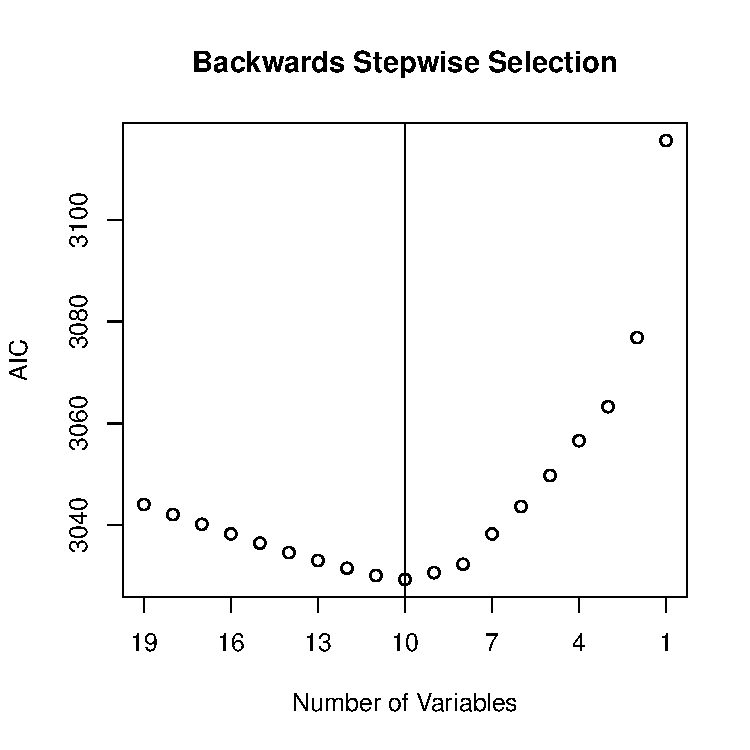
\includegraphics[scale=0.5]{figure/bwdAIC}
\end{figure}
\end{frame}

%--------------------------------------------
\begin{frame}[fragile]
The \texttt{step()} function can be used perform stepwise selection.  The function is convenient since it outputs the selected regression model (an \texttt{lm} object).
\scriptsize
\begin{verbatim}
> lm_full <- lm(Salary ~ ., data=Hitters2)
> lm2 <- step(lm_full)
> summary(lm2)
Coefficients:
              Estimate Std. Error t value Pr(>|t|)    
(Intercept)  162.53544   66.90784   2.429 0.015830 *  
AtBat         -2.16865    0.53630  -4.044 7.00e-05 ***
Hits           6.91802    1.64665   4.201 3.69e-05 ***
Walks          5.77322    1.58483   3.643 0.000327 ***
CAtBat        -0.13008    0.05550  -2.344 0.019858 *  
CRuns          1.40825    0.39040   3.607 0.000373 ***
CRBI           0.77431    0.20961   3.694 0.000271 ***
CWalks        -0.83083    0.26359  -3.152 0.001818 ** 
DivisionW   -112.38006   39.21438  -2.866 0.004511 ** 
PutOuts        0.29737    0.07444   3.995 8.50e-05 ***
Assists        0.28317    0.15766   1.796 0.073673 .  
---
Signif. codes:  0 ‘***’ 0.001 ‘**’ 0.01 ‘*’ 0.05 ‘.’ 0.1 ‘ ’ 1

Residual standard error: 311.8 on 252 degrees of freedom
Multiple R-squared:  0.5405,	Adjusted R-squared:  0.5223 
F-statistic: 29.64 on 10 and 252 DF,  p-value: < 2.2e-16
\end{verbatim}
\end{frame}

%--------------------------------------------------------
\begin{frame}[fragile]
We can also use the \texttt{step()} function to select a model using the BIC by specifying the argument \texttt{k=log(n)} (note by default \texttt{k=2} which specifies the penalty for the AIC).  When using the BIC, 8 predictors are selected (less than AIC).  
\scriptsize
\begin{verbatim}
> n <- nrows(Hitters2)
> lm3 <- step(lm_full, k=log(n))
> summary(lm3)
Coefficients:
              Estimate Std. Error t value Pr(>|t|)    
(Intercept)  117.15204   65.07016   1.800 0.072985 .  
AtBat         -2.03392    0.52282  -3.890 0.000128 ***
Hits           6.85491    1.65215   4.149 4.56e-05 ***
Walks          6.44066    1.52212   4.231 3.25e-05 ***
CRuns          0.70454    0.24869   2.833 0.004981 ** 
CRBI           0.52732    0.18861   2.796 0.005572 ** 
CWalks        -0.80661    0.26395  -3.056 0.002483 ** 
DivisionW   -123.77984   39.28749  -3.151 0.001824 ** 
PutOuts        0.27539    0.07431   3.706 0.000259 ***
---
Signif. codes:  0 ‘***’ 0.001 ‘**’ 0.01 ‘*’ 0.05 ‘.’ 0.1 ‘ ’ 1

Residual standard error: 314.7 on 254 degrees of freedom
Multiple R-squared:  0.5281,	Adjusted R-squared:  0.5133 
F-statistic: 35.54 on 8 and 254 DF,  p-value: < 2.2e-16
\end{verbatim}
\end{frame}

%--------------------------------------------
\begin{frame}{Which Criterion to Use?}
\begin{itemize}
\item AIC and BIC have rigorous theoretical justification in information theory.  Both criterion also generalize for use in multiple logistic regression.
\vspace{10pt}
\item The adjusted-$R^2$, while intuitive, is not as well motivated by theory.
\vspace{10pt}
\item The AIC is probably the most widely used criterion.  BIC might be preferable if you want to select smaller sets of predictors.
\end{itemize}

%--------------------------------------------
\end{frame}
\begin{frame}{Comments}
\begin{itemize}
\item If interpretation is the goal, then automated variable selection methods should not be used as a substitute for thinking about the context of your data and the validity selected model. 
\vspace{5pt}
\begin{itemize}
\item Assess whether the signs and magnitudes of the coefficients make sense in the selected model.  
\item It also might be worthwhile to assess collinearity and to manually remove or combine correlated variables. 
\item Look at scatter plots of the data and residuals plots.  These diagnostics might indicate problems with nonlinearity or nonconstant variance, and thus motivate transformations that fix these issues.
\end{itemize}
\vspace{5pt}
\item If prediction is the goal, then it is recommended to do some form of cross-validation.  Withhold some data and evaluate how well the model performs on that withheld, validation set (topic for a future class).
\end{itemize}
\end{frame}


\end{document}
